\section{Results}

\subsection{Model Simulation}
    \paragraph{Current Dynamics}

    During periods of minimum inhibition, a set of populations displays a positive current corresponding to one memory.
    Meanwhile, the remaining populations have negative current, meaning other memories are not being recalled.

    At inhibition maxima, transitions between attractors may happen, with a new set of neuron populations firing at the next inhibition minimum.
    Transitions are observed when current values near inhibition minima, where values are close enough for the noise to drive changes between limit cycles (Figure \ref{fig:currents}).
    
    \begin{figure}
        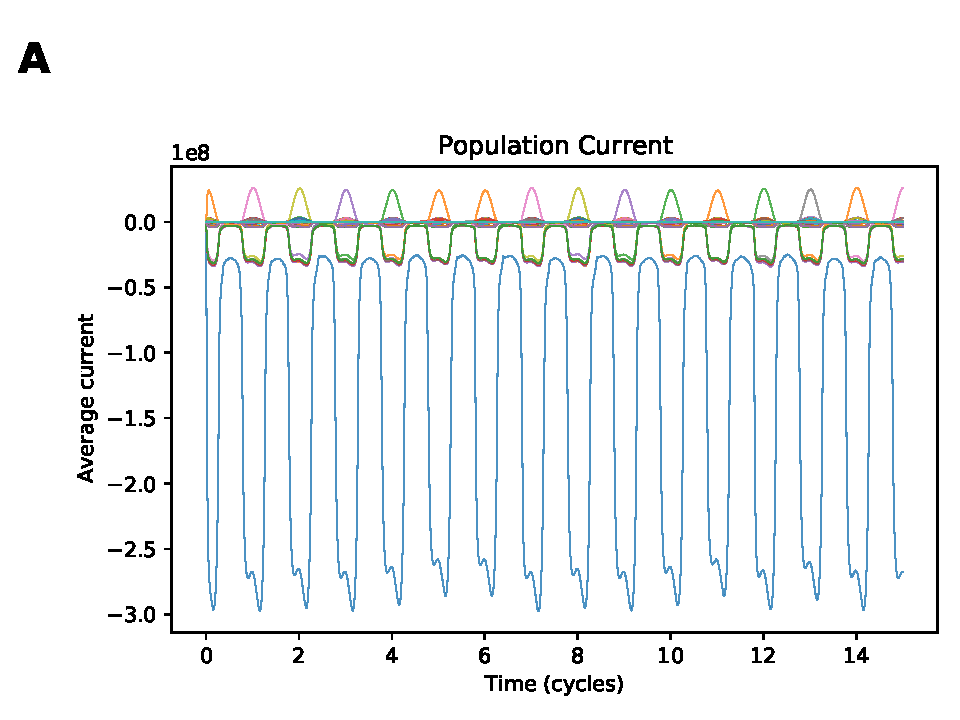
\includegraphics[width=\textwidth]{graphics/currents_populations.pdf}
        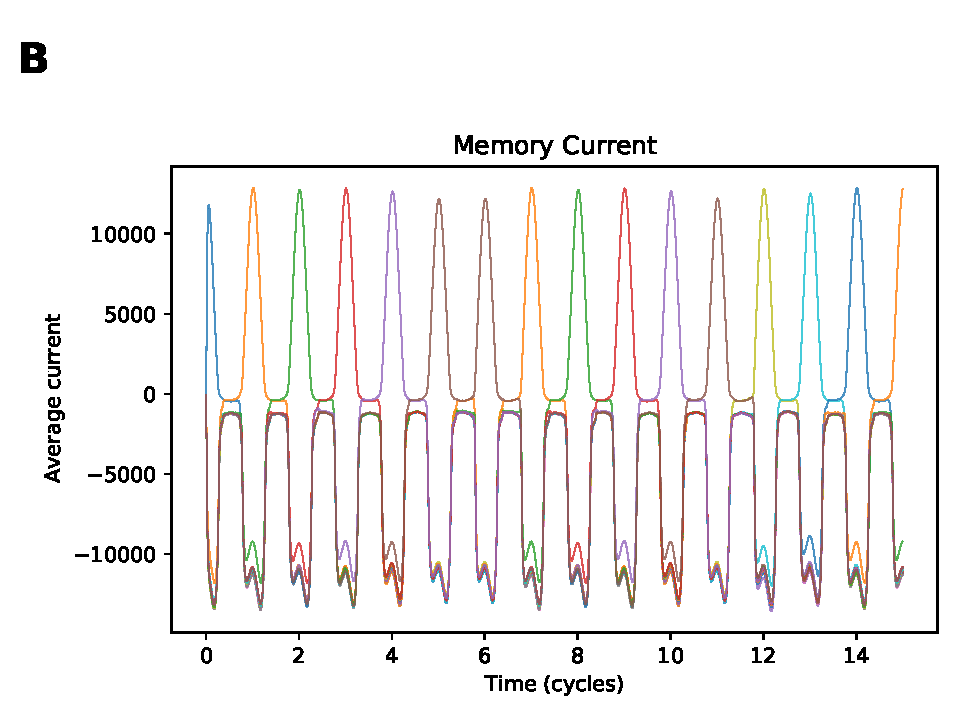
\includegraphics[width=\textwidth]{graphics/currents_memories.pdf}
        \caption{
        Currents.
        \textbf{A.} Currents of each population of neurons over time.
        \textbf{B.} Memories activation over time.
        Each color represents a different population (A) or memory (B).
        Axis units are arbitrary.
        }
        \label{fig:currents}
    \end{figure}
    
    \paragraph{Firing Rates}

    Currents are subjected to a step function to calculate firing rates.
    The curve shape of the latter is then closely related to the positive domain of current values over time.
    Firing rates above \(r_{recall}\) indicate that a memory was recalled.
    Different memories are recalled at times corresponding to minimum values of inhibition.
    Transitions may happen between memory items or attractors in periods of minimum inhibition (Figure \ref{fig:firing_rates}).

    \begin{figure}
        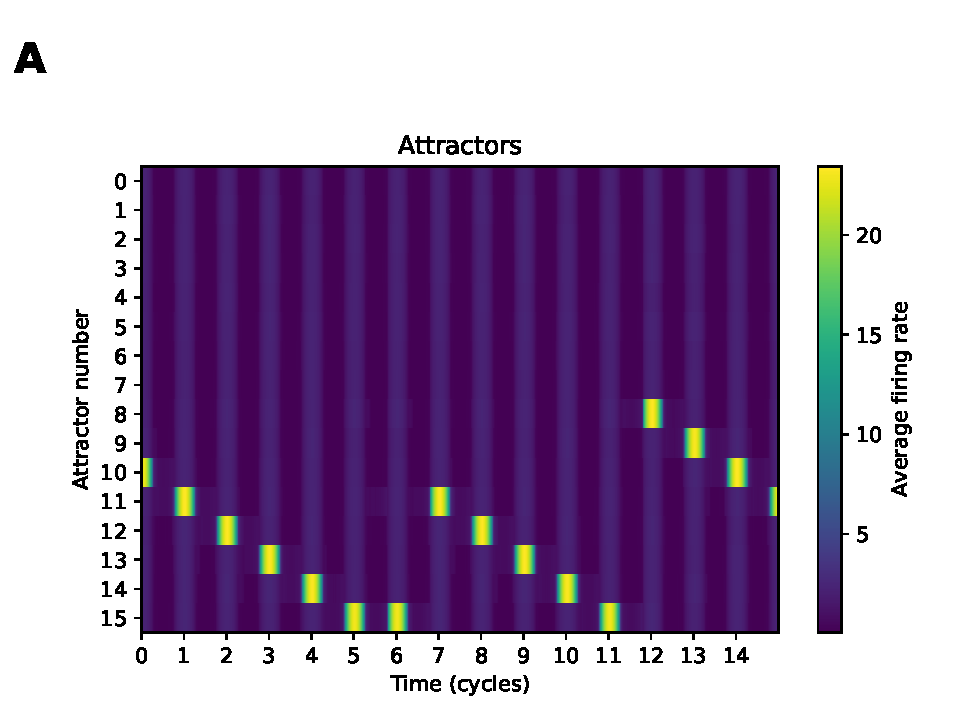
\includegraphics[width=\textwidth]{graphics/firing_rates_attractors.pdf}
        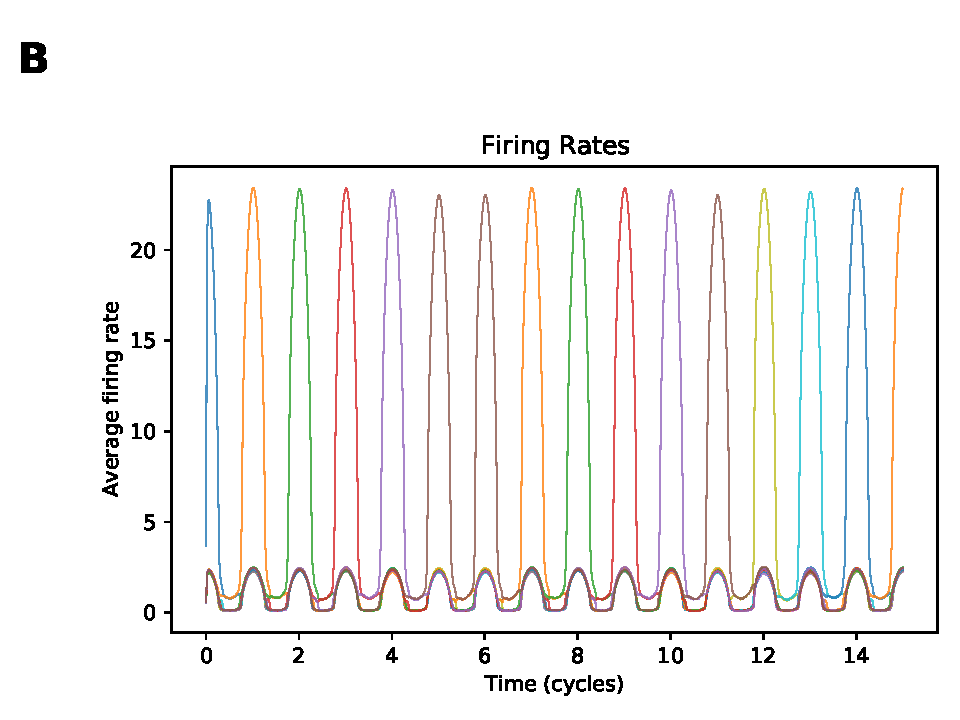
\includegraphics[width=\textwidth]{graphics/firing_rates_lines.pdf}
        \caption{
        Network dynamics.
        \textbf{A.} Attractor states.
        The color indicates the firing rate.
        \textbf{B.} Average firing rates corresponding to each memory pattern.
        Each color represents a population.
        Transitions may happen between memory items or attractors in periods of minimum inhibition.
        Axis units are arbitrary.
        }
        \label{fig:firing_rates}
    \end{figure}
    
    \paragraph{Inhibition}

    The sine wave function provides the network with oscillatory inhibition necessary for its dynamics.
    Values have to be adequately scaled to induce the appropriate network behavior of memory recall and transitions between attractors (Figure \ref{fig:inhibition}).

    \begin{figure}
        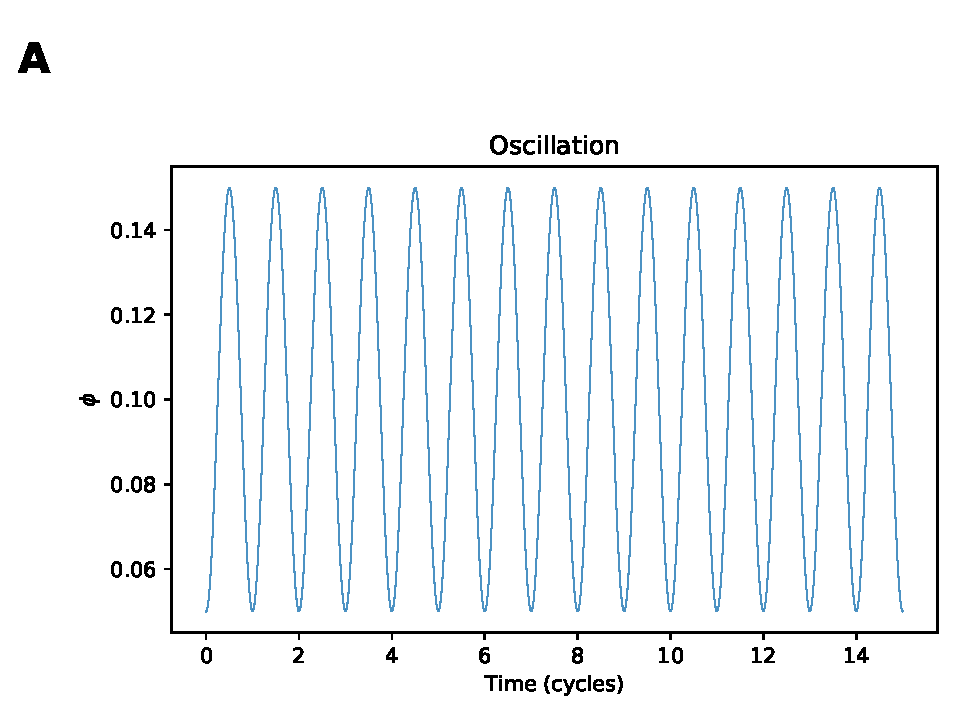
\includegraphics[width=\textwidth]{graphics/oscillation.pdf}
        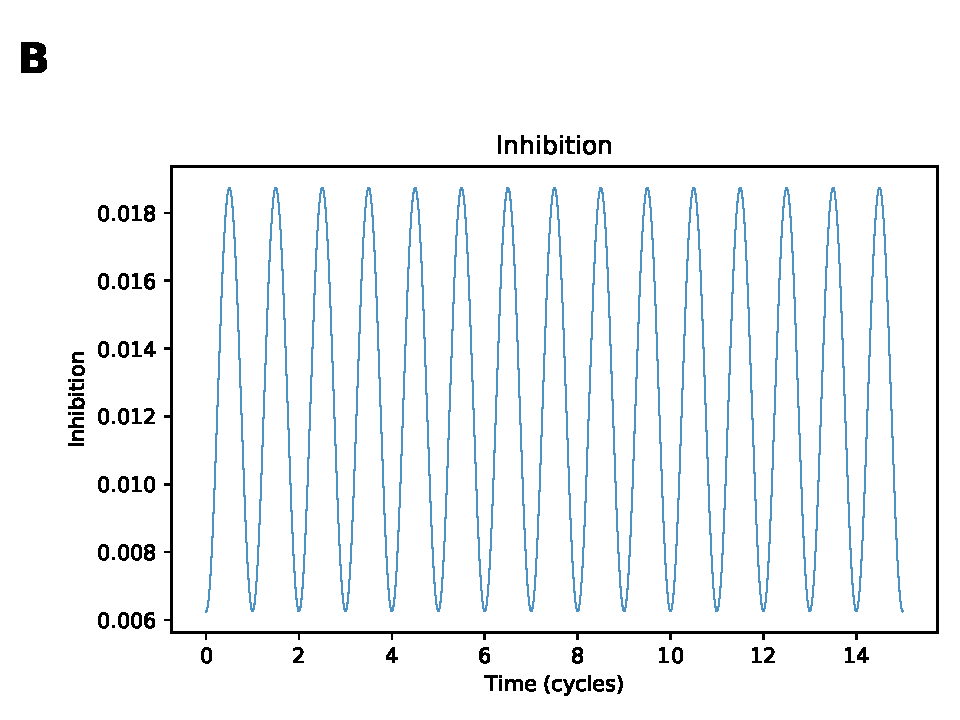
\includegraphics[width=\textwidth]{graphics/inhibition.pdf}
        \caption{
        \(\phi\) function and inhibition.
        \textbf{A.} Sine wave function values over time, which need to be scaled to have an adequate inhibitory effect on the network.
        \textbf{B.} Inhibition over time, driving the periodic behavior of the network.
        Axis units are arbitrary.
        }
        \label{fig:inhibition}
    \end{figure}
    \paragraph{Weights}

    Weights show the strength of the connection between elements \(i j\) of the matrix.
    In the model, three different weight matrices are presented, accounting for the regular connectivity between neuron populations, but also considering item contiguity or associations between
    Weight values change according to the parameters of excitation, forward, and backward contiguity (Figure \ref{fig:weights}).
        
    \begin{figure}
        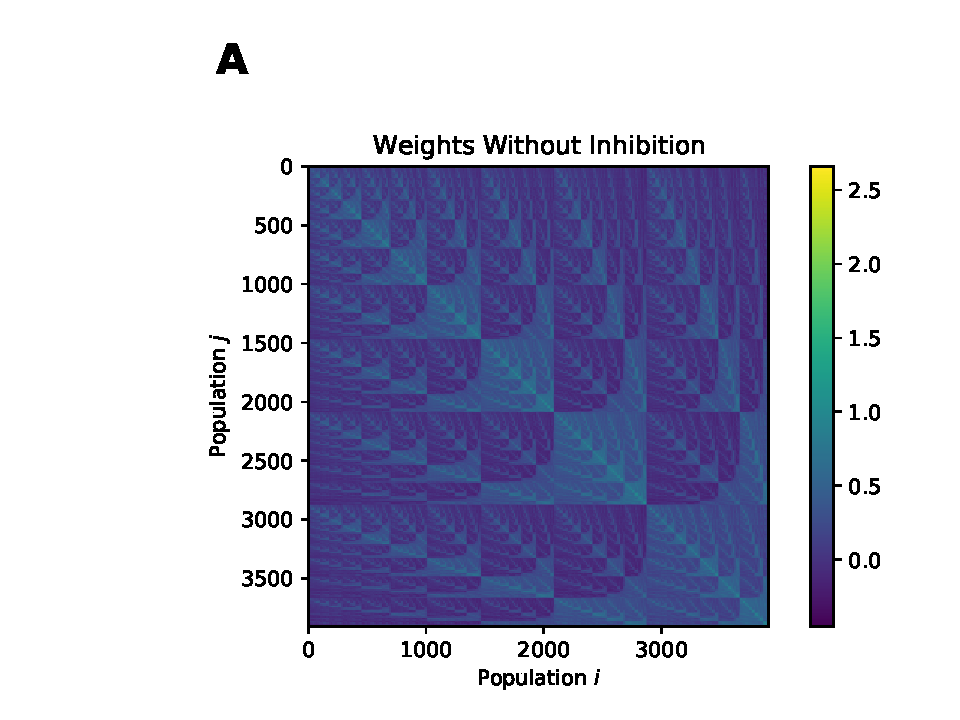
\includegraphics[width=0.5\textwidth]{graphics/weights_without_inhibition.pdf}
        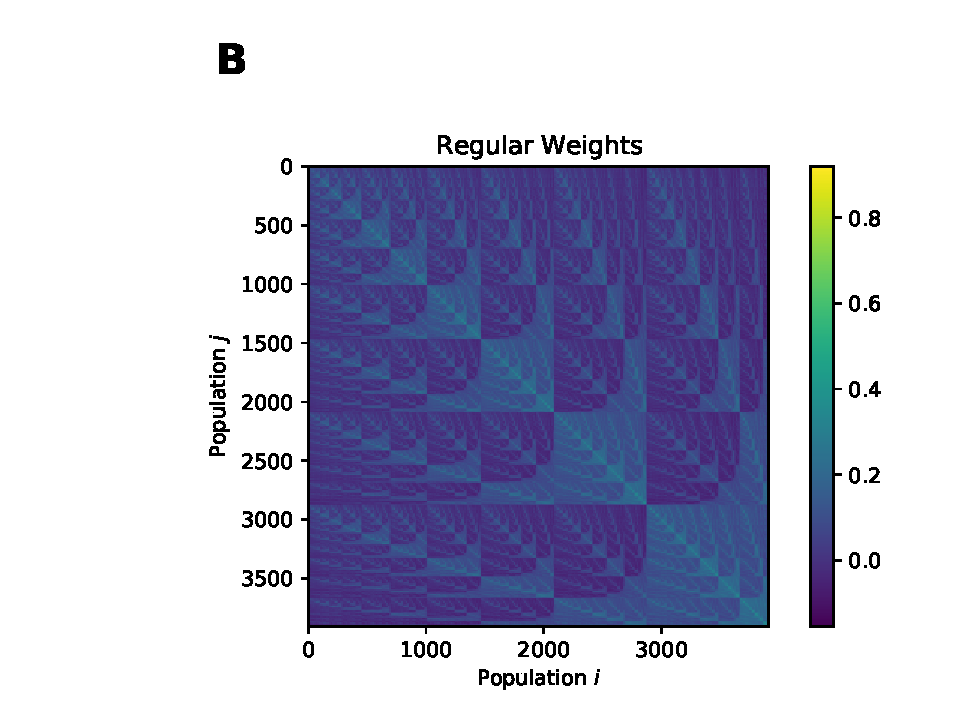
\includegraphics[width=0.5\textwidth]{graphics/weights_reg.pdf}
        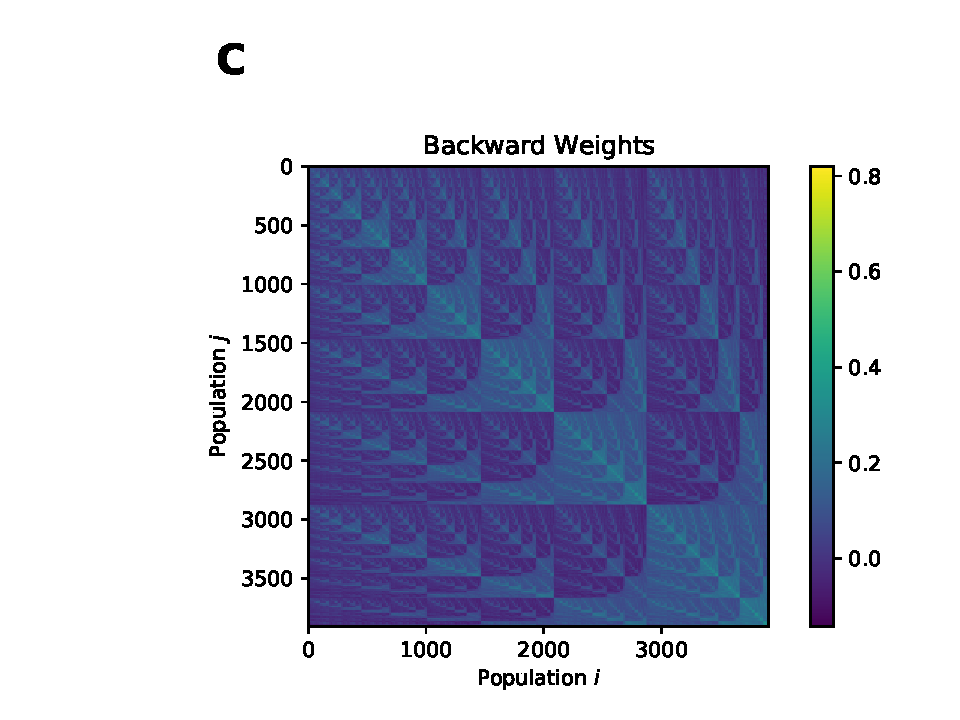
\includegraphics[width=0.5\textwidth]{graphics/weights_back.pdf}
        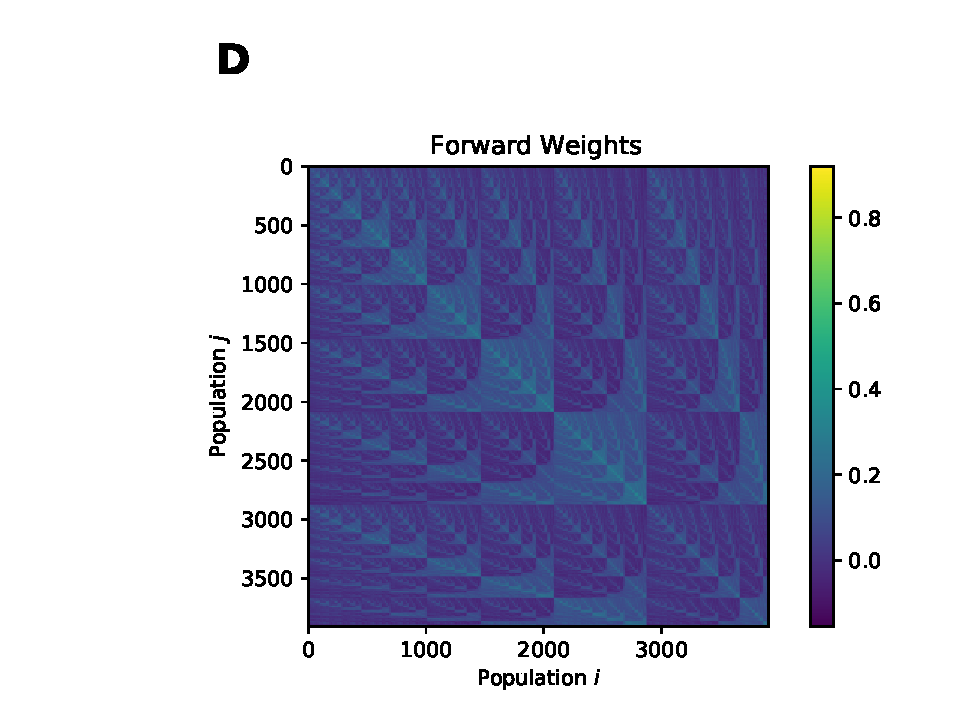
\includegraphics[width=0.5\textwidth]{graphics/weights_forth.pdf}
        \caption{
        The strength of the connection between network elements is shown, with higher values in the color scale indicating stronger association (see color bars).
        \textbf{A.} Weight matrix previous to the addition of the inhibitory terms.
        \textbf{B.} Weights after adding inhibition.
        \textbf{C.} Weights corresponding to backward item contiguity.
        \textbf{D.} Weights corresponding to item contiguity.
        Values before applying inhibition (A) are higher than those in ``regular'' and contiguity connectivity (B, C, D).
        Also, the overall distribution of values is shifted with respect to the main diagonal in backward (forward) contiguity connectivity, as the connection links to the previous (next) unit.
        Axis units are arbitrary.
        }
        \label{fig:weights}
    \end{figure}

    \paragraph{Noise}

    Uncorrelated Gaussian noise is calculated for each population of neurons.
    The range of values is critical for the network to be successfully simulated, observing the transition between attractors (Figure \ref{fig:noise}).

    \begin{figure}
        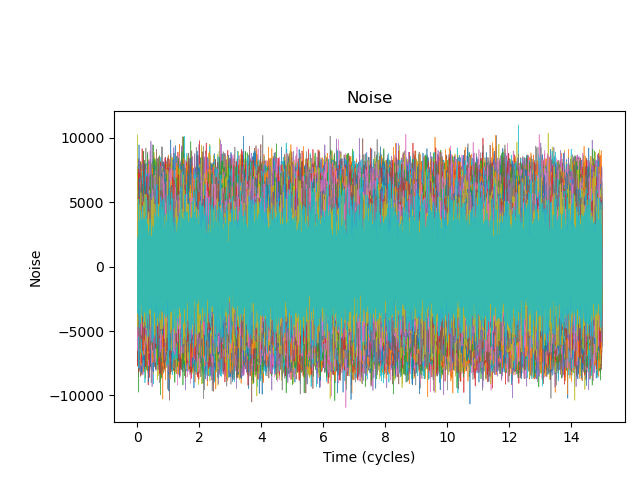
\includegraphics[width=\textwidth]{graphics/noise.png}
        \caption{
        Noise for all populations,
        with a different color for each population of neurons.
        Values are centered around 0 (the mean of the distribution), and maximum and minimum values fall within a range that allows attractor transitions without distorting basic network dynamics.
        Axis units are arbitrary.
        }
        \label{fig:noise}
    \end{figure}

\subsection{Recall Analysis}
    \paragraph{Temporal Properties of Recall}

    Recall of new memories progressively slows down with time, while still possible even at later time cycles, even observing a sharp increase in recalls in the last iterations.
    Most transitions occur after one time step (IRT = 0), while there is some variability in the distribution.
    As time passes, the average IRT is likely to decrease due to these rapid memory transitions (Figure \ref{fig:temporal_properties_recall}).

    \paragraph{Probability of Recall}

    The frequency of recall monotonically increases with memory size, as more overlaps between large memories are expected.
    As time passes, the average IRT is likely to decrease due to these rapid memory transitions (Figure \ref{fig:probability_recall}).
    Differences in the number of points of the figure compared to the original article are likely due to binning and not due to a change in dynamics. 
    
    \paragraph{Memory Transitions}
    
    More similar memories are expected to be recalled more often.
    This effect is observed as most transitions occur between the most similar memories.
    There is also a higher transition rate between memories with a lower intersection size between them.
    This leads to fast transitions, or lower IRT values for more similar memories (Figure \ref{fig:recall_performance_transitions}).

    \paragraph{Recall Performance and Parameters}

    Average total number of memories recalled by 100 networks for 100 different values of forward contiguity and noise variance (Figure \ref{fig:recall_performance_params}).
    Networks recall more words on average with monotonically increasing 
    with the value of noise variance \(\sigma^{2}\) until saturation.
    The performance also increases along with forward contiguity \(\kappa_{f}\) until saturation, followed by a decrease in recalls.
    At this point, the contiguity term likely overcomes noise as the drive for memory transitions.
    An additional evaluation focuses on lower forward contiguity values \(\kappa_{f}\).
    This supports that the dynamics at the lowest values of \(\kappa_{f}\) in the previous figure are due to its relationship with \(\kappa_{b}\), and not entirely due to randomness.
    A drop in performance is seen as values get closer to backward contiguity \(\kappa_{b} = 850\), rising again afterward.
        
    \begin{figure}
        \centering
        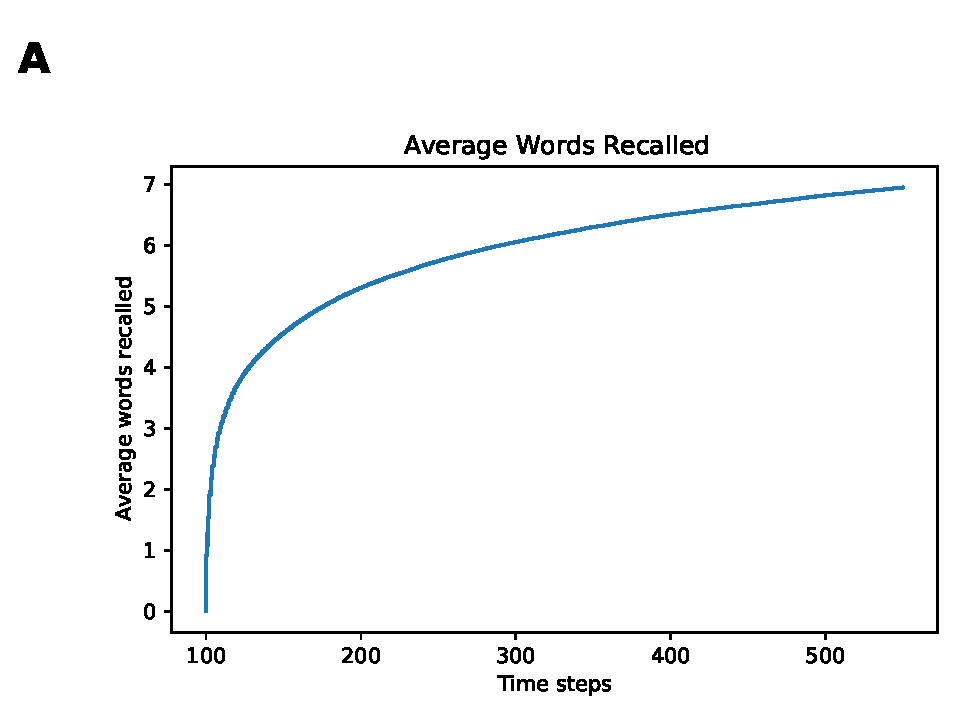
\includegraphics[width=.69\textwidth]{graphics/time_words_recalled.pdf}
        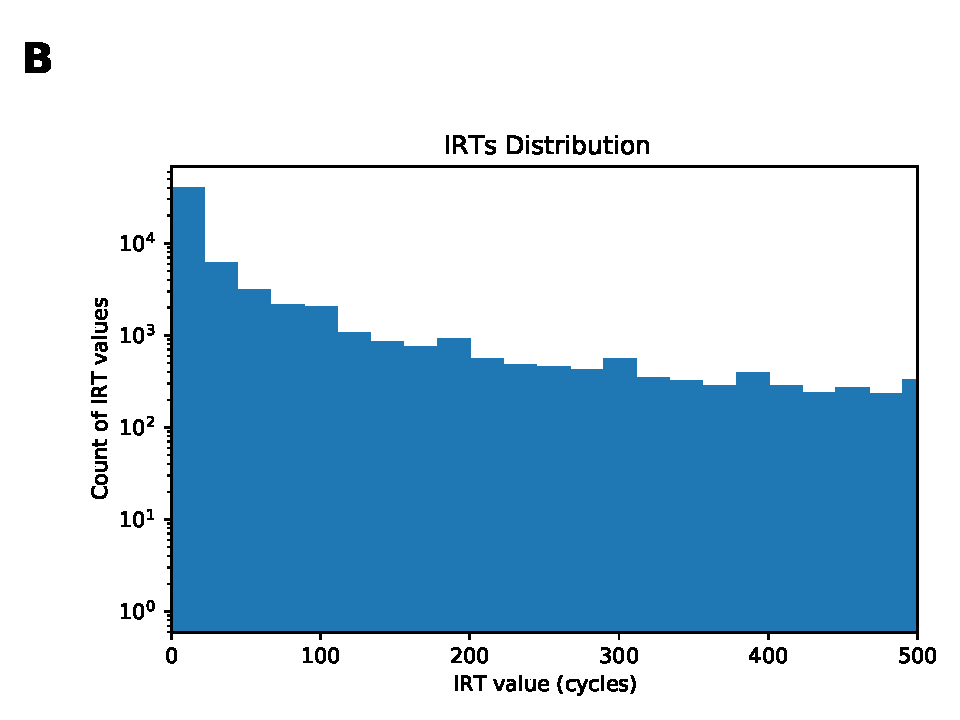
\includegraphics[width=.69\textwidth]{graphics/time_distribution_irt.pdf}
        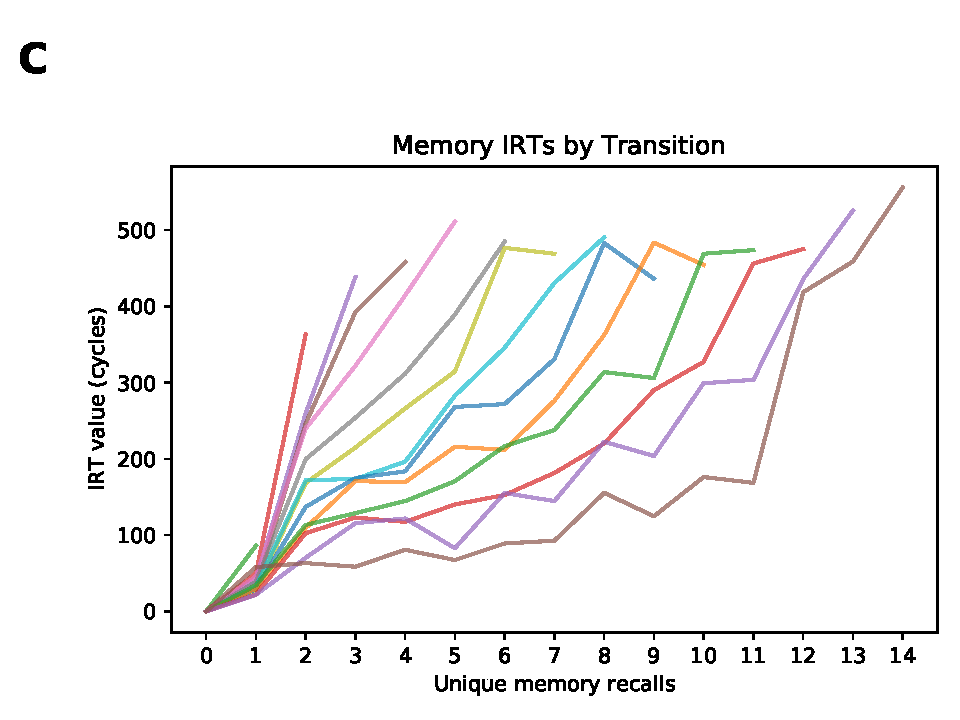
\includegraphics[width=.69\textwidth]{graphics/time_average_irt.pdf}
        \caption{
        Temporal properties of recall.
        \textbf{A.} Cumulative sum of new memory recalls: a memory is added only the first time it is recalled over time.
        \textbf{B.} Number of occurrences of IRTs ordered by their size in time cycles.
        \textbf{C.} Average IRT values divided by the number of transitions for each line (memory).
        }
        \label{fig:temporal_properties_recall}
    \end{figure}
    \clearpage
    
    \begin{figure}
        \centering
        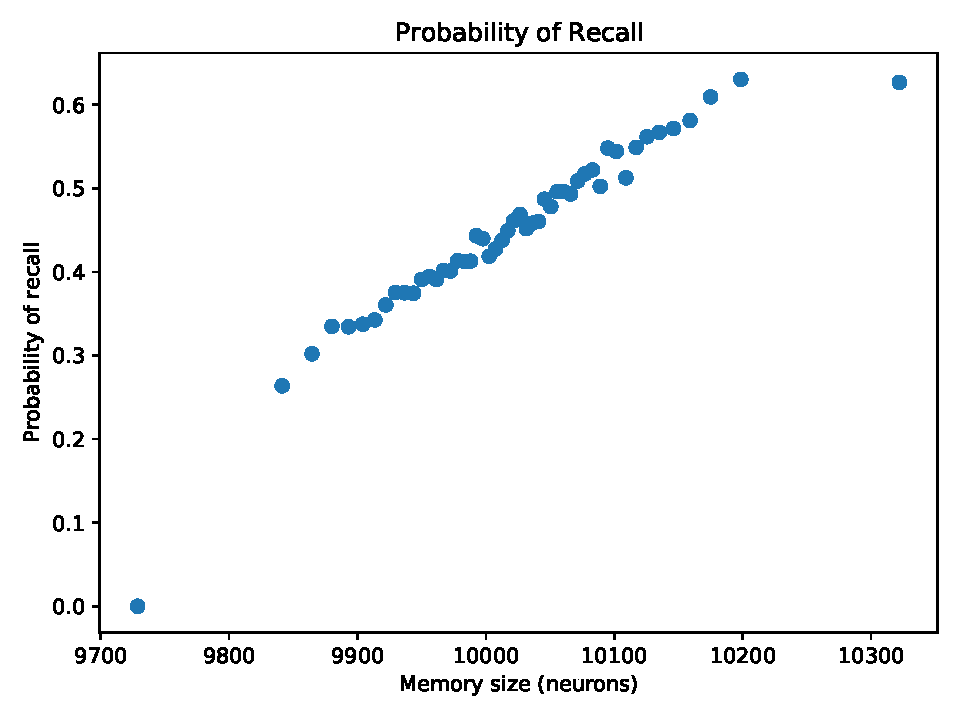
\includegraphics[width=\textwidth]{graphics/probability_recall.pdf}
        \caption{
        Frequency of memory recalls according to their size.
        Larger memories are recalled more often.
        }
        \label{fig:probability_recall}
    \end{figure}
    \clearpage
    
    \begin{figure}
        \centering
        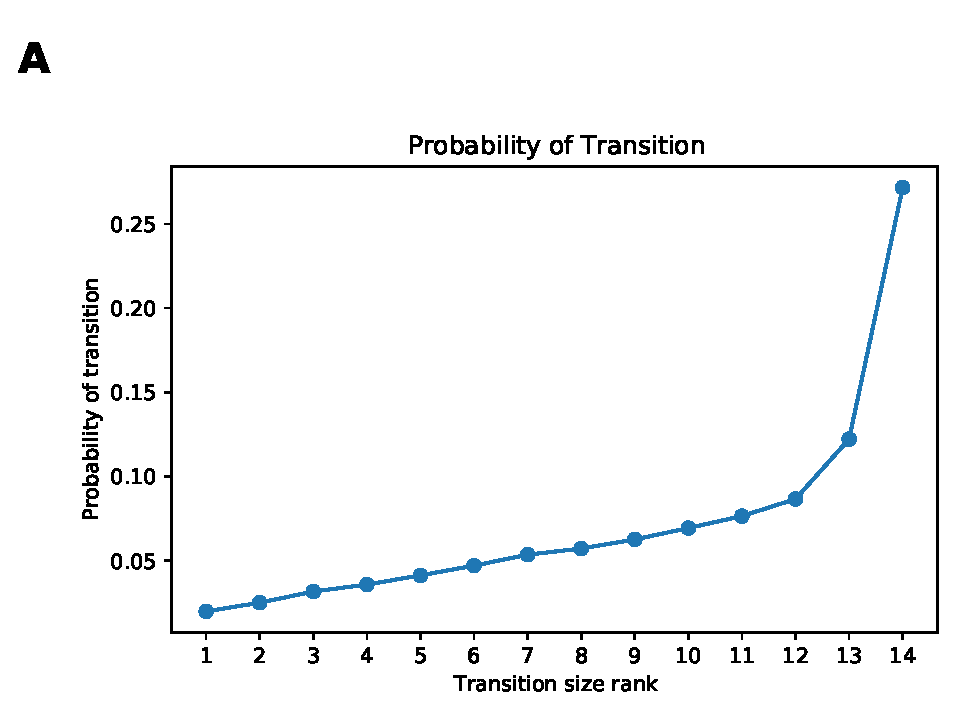
\includegraphics[width=.68\textwidth]{graphics/transitions_probability.pdf}
        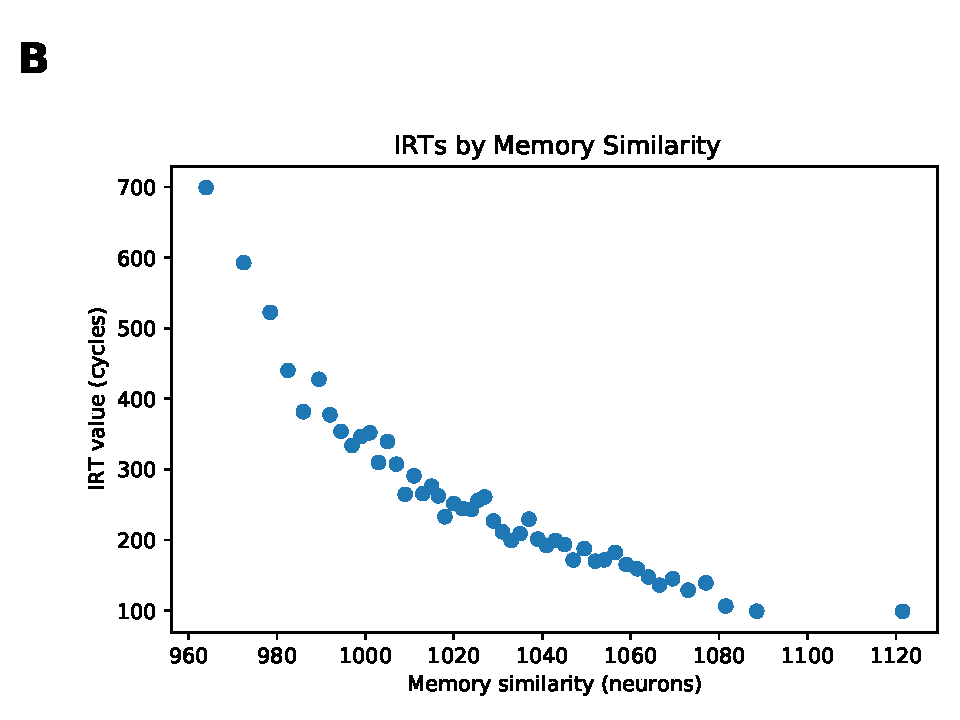
\includegraphics[width=.68\textwidth]{graphics/transitions_irt.pdf}
        \caption{
        Influence of memory intersection sizes in the recall process.
        \textbf{A.} Proportion of transitions ranked in 15 groups of the same size, from less to more similar.
        \textbf{B.} Average IRT as a function of the intersection size in neurons
        }
        \label{fig:recall_performance_transitions}
    \end{figure}
    \clearpage
    
    \begin{figure}
        \centering
        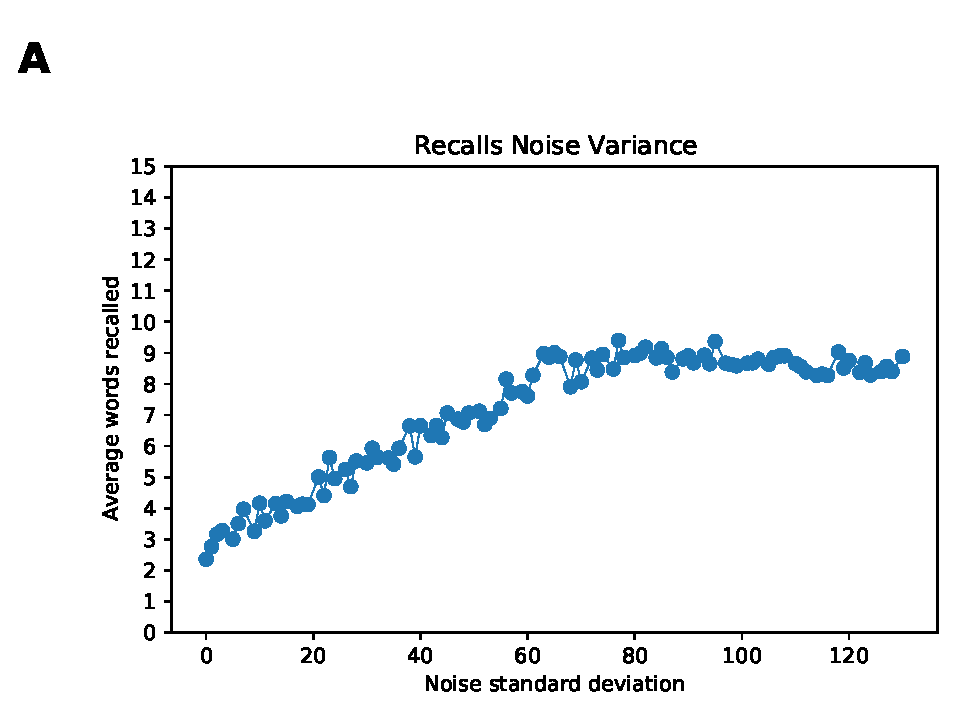
\includegraphics[width=.68\textwidth]{graphics/noise_var.pdf}
        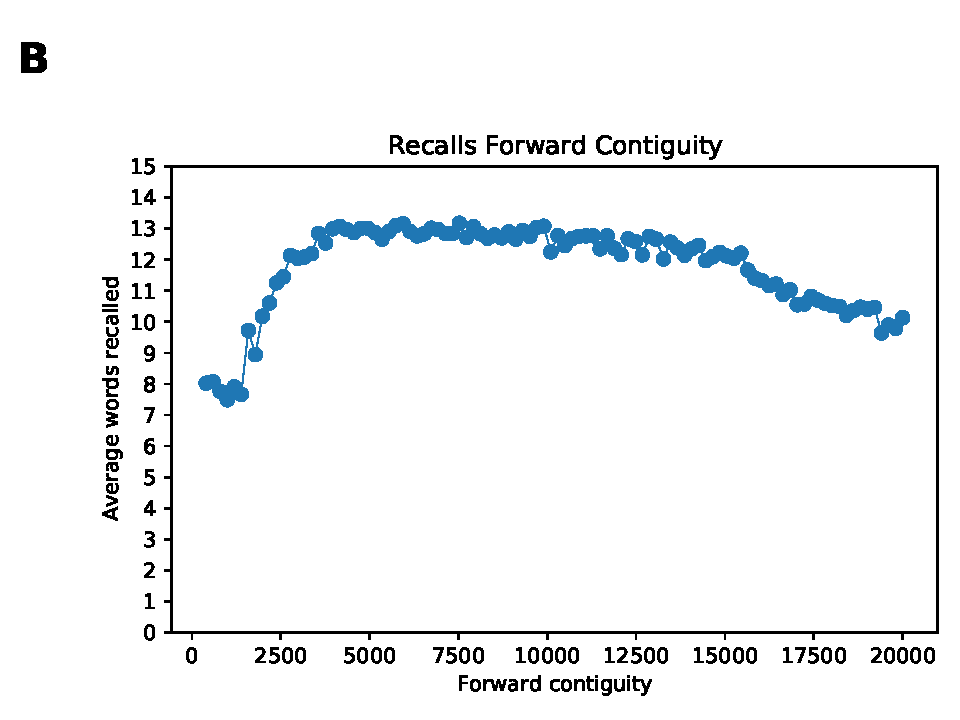
\includegraphics[width=.68\textwidth]{graphics/cont_forth.pdf}
        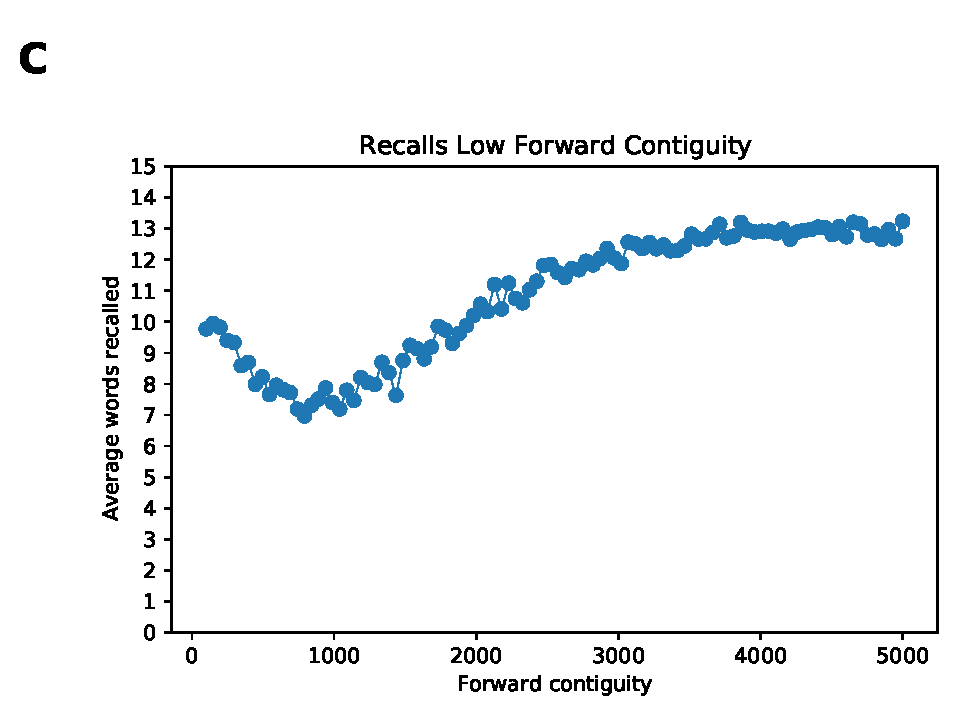
\includegraphics[width=.68\textwidth]{graphics/cont_forth_low.pdf}
        \caption{
        Recall performance with varying forward contiguity and noise variance.
        \textbf{A.} Performance when varying the value of noise variance \(\sigma^{2}\) between 0 and 130.
        \textbf{B.} Performance when varying the value of forward contiguity \(\kappa_{f}\) between 850 and 20,000.
        \textbf{C.} Recall performance with varying forward contiguity \(\kappa_{f}\) between 100 and 5,000.
        A drop in performance is seen as values get closer to backward contiguity \(\kappa_{b} = 850\), rising again afterward.
        }
        \label{fig:recall_performance_params}
    \end{figure}
    \clearpage